\documentclass[aspectratio=169]{beamer}

\usetheme{default}
\usecolortheme{dove}

\setbeamertemplate{navigation symbols}{}
\setbeamertemplate{footline}{%
  \hfill{\large\insertframenumber\,/\,\inserttotalframenumber}\hspace{0.8em}\vspace{0.5em}%
}

\definecolor{popblue}{RGB}{52, 101, 164}
\definecolor{sampred}{RGB}{204, 0, 0}
\definecolor{paramgreen}{RGB}{0, 140, 70}
\definecolor{warnred}{RGB}{180, 40, 40}
\definecolor{orange1}{RGB}{220, 120, 0}
\definecolor{violet1}{RGB}{120, 50, 160}
\definecolor{lightbg}{RGB}{245, 245, 250}

\setbeamercolor{frametitle}{fg=popblue}
\setbeamercolor{title}{fg=popblue}

\usepackage{pgfplots}
\usepackage{tikz}
\usetikzlibrary{shapes, arrows.meta, positioning, calc, decorations.pathreplacing, patterns}
\pgfplotsset{compat=1.18}
\usepackage{amsmath, amssymb}
\usepackage{pifont}
\usepackage{colortbl}
\usepackage{fontenc}

\title{Lecture 14: Causal Inference}
\subtitle{From ``What Happened?'' to ``What Would Happen If\ldots?''}
\date{}

\begin{document}

% ============================================================
\begin{frame}
\titlepage
\end{frame}

% ============================================================
\begin{frame}
\frametitle{Previously, on Lecture 13\ldots}

\begin{center}
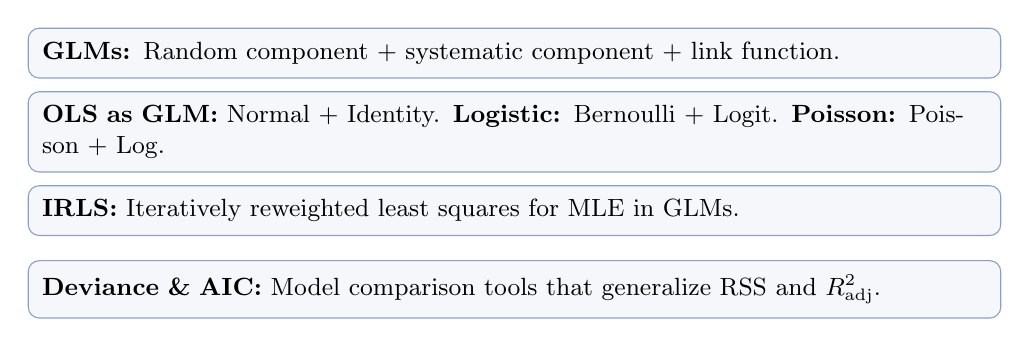
\begin{tikzpicture}[
  sbox/.style={draw=popblue!60, fill=popblue!5, rounded corners=4pt, text width=12cm, minimum height=0.5cm, align=left, inner sep=5pt, font=\small}
]
  \node[sbox] at (0, 2.0) {\textbf{GLMs:} Random component + systematic component + link function.};
  \node[sbox] at (0, 1.0) {\textbf{OLS as GLM:} Normal + Identity. \textbf{Logistic:} Bernoulli + Logit. \textbf{Poisson:} Poisson + Log.};
  \node[sbox] at (0, 0.0) {\textbf{IRLS:} Iteratively reweighted least squares for MLE in GLMs.};
  \node[sbox] at (0,-1.0) {\textbf{Deviance \& AIC:} Model comparison tools that generalize RSS and $R^2_\text{adj}$.};
\end{tikzpicture}
\end{center}

\vspace{0.3cm}
\begin{center}
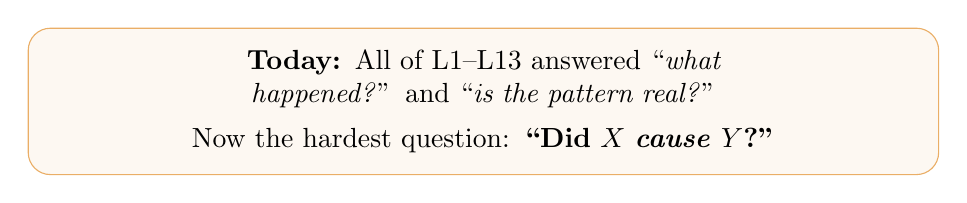
\begin{tikzpicture}
  \node[draw=orange1!60, fill=orange1!5, rounded corners=8pt, text width=11cm, align=center, inner sep=8pt] {
    \textbf{Today:} All of L1--L13 answered ``\textit{what happened?}'' and ``\textit{is the pattern real?}''\\[4pt]
    Now the hardest question: \textbf{``Did $X$ \textit{cause} $Y$?''}
  };
\end{tikzpicture}
\end{center}
\end{frame}

% ============================================================
\begin{frame}
\frametitle{Outline}
\tableofcontents
\end{frame}

% ============================================================
% PART I: CORRELATION ≠ CAUSATION
% ============================================================
\section{Correlation $\neq$ Causation}

\begin{frame}
\begin{center}
  \vspace{1.5cm}
  {\Huge\bfseries\textcolor{popblue}{Part I: Correlation $\neq$ Causation}}

  \vspace{0.8cm}
  {\large The most important sentence in statistics}
\end{center}
\end{frame}

\begin{frame}
\frametitle{Spurious Correlations}

\begin{center}
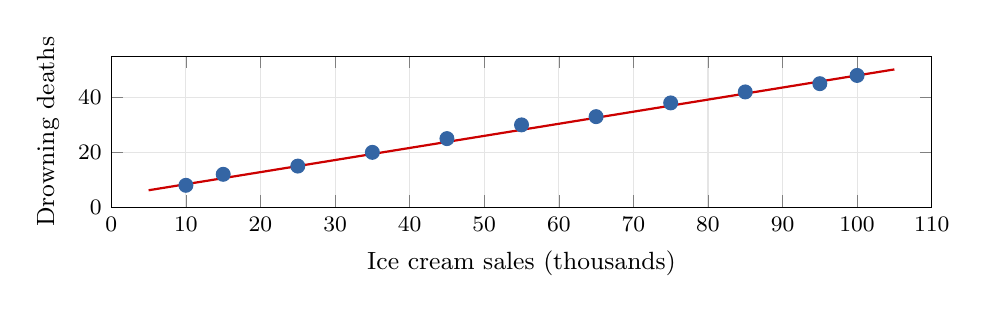
\begin{tikzpicture}
\begin{axis}[
  width=12cm, height=3.5cm,
  xlabel={Ice cream sales (thousands)},
  ylabel={Drowning deaths},
  xmin=0, xmax=110, ymin=0, ymax=55,
  grid=major, grid style={gray!20},
  every axis label/.style={font=\small},
  tick label style={font=\footnotesize}
]
  \addplot[only marks, mark=*, mark size=2.5pt, popblue] coordinates {
    (10,8) (15,12) (25,15) (35,20) (45,25) (55,30)
    (65,33) (75,38) (85,42) (95,45) (100,48)
  };
  \addplot[sampred, thick, domain=5:105] {0.44*x + 4};
\end{axis}
\end{tikzpicture}
\end{center}

\vspace{0.05cm}
\begin{center}

\begin{tikzpicture}
  \node[draw=warnred, fill=warnred!5, rounded corners=5pt, text width=11cm, align=center, inner sep=5pt, font=\small] {
    $r = 0.95$, $p < 0.001$. Banning ice cream saves lives?
    \textbf{No.} A \textbf{confounder} (hot weather) drives both.
  };
\end{tikzpicture}
\end{center}

\vspace{0.05cm}
\begin{center}
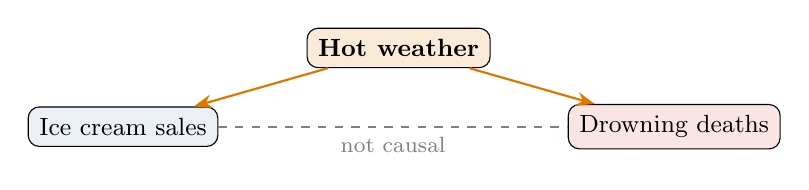
\begin{tikzpicture}[
  cnode/.style={draw, rounded corners=4pt, inner sep=4pt, font=\small, minimum width=2.2cm, align=center}
]
  \node[cnode, fill=orange1!15] (Z) at (0, 1.0) {\textbf{Hot weather}};
  \node[cnode, fill=popblue!10] (X) at (-3.5, 0) {Ice cream sales};
  \node[cnode, fill=sampred!10] (Y) at (3.5, 0) {Drowning deaths};
  \draw[-{Stealth}, thick, orange1] (Z) -- (X);
  \draw[-{Stealth}, thick, orange1] (Z) -- (Y);
  \draw[dashed, gray, thick] (X) -- (Y) node[midway, below, font=\footnotesize, gray] {not causal};
\end{tikzpicture}
\end{center}
\end{frame}

\begin{frame}
\frametitle{Three Reasons Correlation $\neq$ Causation}

\begin{center}
\begin{tikzpicture}[
  rbox/.style={draw, rounded corners=5pt, text width=3.4cm, align=center, inner sep=4pt, font=\small, minimum height=2.2cm},
  arr/.style={-{Stealth}, thick}
]
  % Confounding
  \node[rbox, fill=orange1!10] (c) at (-5, 0) {
    \textbf{1. Confounding}\\[2pt]
    \begin{tikzpicture}[scale=0.5]
      \node[draw, circle, fill=orange1!20, inner sep=2pt, font=\scriptsize] (z) at (0,1.2) {$Z$};
      \node[draw, circle, fill=popblue!15, inner sep=2pt, font=\scriptsize] (x) at (-1.2,0) {$X$};
      \node[draw, circle, fill=sampred!15, inner sep=2pt, font=\scriptsize] (y) at (1.2,0) {$Y$};
      \draw[arr, orange1, scale=0.8] (z) -- (x);
      \draw[arr, orange1, scale=0.8] (z) -- (y);
    \end{tikzpicture}\\
    {\footnotesize $Z$ causes both}
  };
  % Reverse causation
  \node[rbox, fill=sampred!10] (r) at (0, 0) {
    \textbf{2. Reverse causation}\\[2pt]
    \begin{tikzpicture}[scale=0.5]
      \node[draw, circle, fill=popblue!15, inner sep=2pt, font=\scriptsize] (x) at (-1.2,0.5) {$X$};
      \node[draw, circle, fill=sampred!15, inner sep=2pt, font=\scriptsize] (y) at (1.2,0.5) {$Y$};
      \draw[arr, sampred] (y) -- (x);
    \end{tikzpicture}\\
    {\footnotesize $Y$ causes $X$}
  };
  % Collider
  \node[rbox, fill=violet1!10] (col) at (5, 0) {
    \textbf{3. Collider bias}\\[2pt]
    \begin{tikzpicture}[scale=0.5]
      \node[draw, circle, fill=popblue!15, inner sep=2pt, font=\scriptsize] (x) at (-1.2,1.2) {$X$};
      \node[draw, circle, fill=sampred!15, inner sep=2pt, font=\scriptsize] (y) at (1.2,1.2) {$Y$};
      \node[draw, circle, fill=violet1!20, inner sep=2pt, font=\scriptsize] (c) at (0,0) {$C$};
      \draw[arr, popblue] (x) -- (c);
      \draw[arr, sampred] (y) -- (c);
    \end{tikzpicture}\\
    {\footnotesize Conditioning on $C$\\creates bias}
  };
\end{tikzpicture}
\end{center}

\vspace{0.1cm}
\begin{center}
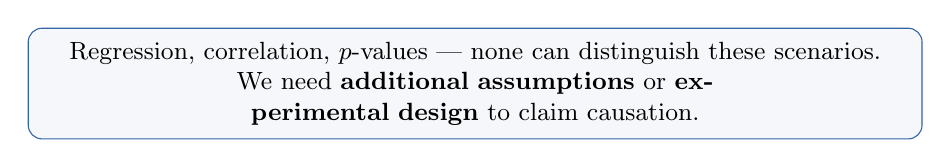
\begin{tikzpicture}
  \node[draw=popblue, fill=popblue!5, rounded corners=5pt, text width=11cm, align=center, inner sep=5pt, font=\small] {
    Regression, correlation, $p$-values --- none can distinguish these scenarios.\\
    We need \textbf{additional assumptions} or \textbf{experimental design} to claim causation.
  };
\end{tikzpicture}
\end{center}
\end{frame}

% ============================================================
% PART II: THE GOLD STANDARD — RCTs
% ============================================================
\section{Randomized Experiments}

\begin{frame}
\begin{center}
  \vspace{1.5cm}
  {\Huge\bfseries\textcolor{popblue}{Part II: The Gold Standard}}

  \vspace{0.8cm}
  {\large Randomized controlled trials (RCTs)}
\end{center}
\end{frame}

\begin{frame}
\frametitle{Why Randomization Works}

\begin{center}
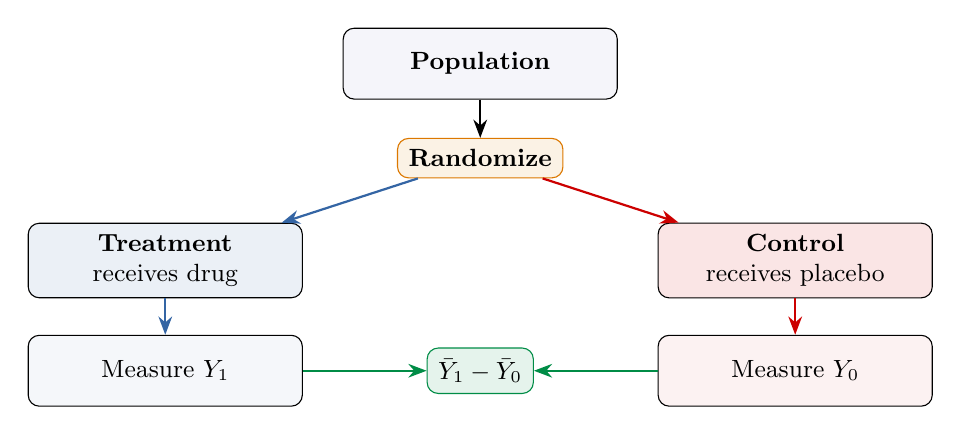
\begin{tikzpicture}[
  bx/.style={draw, rounded corners=4pt, text width=3.2cm, align=center, inner sep=4pt, font=\small, minimum height=0.9cm}
]
  % Population
  \node[bx, fill=lightbg] (pop) at (0, 2.5) {\textbf{Population}};

  % Randomize
  \node[draw=orange1, fill=orange1!10, rounded corners=4pt, inner sep=4pt, font=\small\bfseries] (rand) at (0, 1.3) {Randomize};

  % Two groups
  \node[bx, fill=popblue!10] (treat) at (-4, 0) {\textbf{Treatment}\\receives drug};
  \node[bx, fill=sampred!10] (ctrl) at (4, 0) {\textbf{Control}\\receives placebo};

  % Outcomes
  \node[bx, fill=popblue!5] (y1) at (-4, -1.4) {Measure $Y_1$};
  \node[bx, fill=sampred!5] (y0) at (4, -1.4) {Measure $Y_0$};

  % Compare
  \node[draw=paramgreen, fill=paramgreen!10, rounded corners=4pt, inner sep=4pt, font=\small\bfseries] (comp) at (0, -1.4) {$\bar{Y}_1 - \bar{Y}_0$};

  \draw[-{Stealth}, thick] (pop) -- (rand);
  \draw[-{Stealth}, thick, popblue] (rand) -- (treat);
  \draw[-{Stealth}, thick, sampred] (rand) -- (ctrl);
  \draw[-{Stealth}, thick, popblue] (treat) -- (y1);
  \draw[-{Stealth}, thick, sampred] (ctrl) -- (y0);
  \draw[-{Stealth}, thick, paramgreen] (y1) -- (comp);
  \draw[-{Stealth}, thick, paramgreen] (y0) -- (comp);
\end{tikzpicture}
\end{center}

\vspace{0.1cm}
\begin{center}
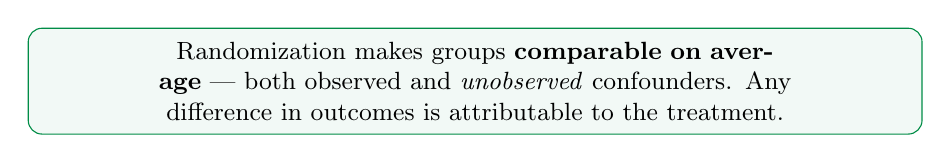
\begin{tikzpicture}
  \node[draw=paramgreen, fill=paramgreen!5, rounded corners=5pt, text width=11cm, align=center, inner sep=5pt, font=\small] {
    Randomization makes groups \textbf{comparable on average} --- both observed and \textit{unobserved} confounders.
    Any difference in outcomes is attributable to the treatment.
  };
\end{tikzpicture}
\end{center}
\end{frame}

\begin{frame}
\frametitle{From A/B Tests to RCTs}
\framesubtitle{Connection to L11}

\begin{center}
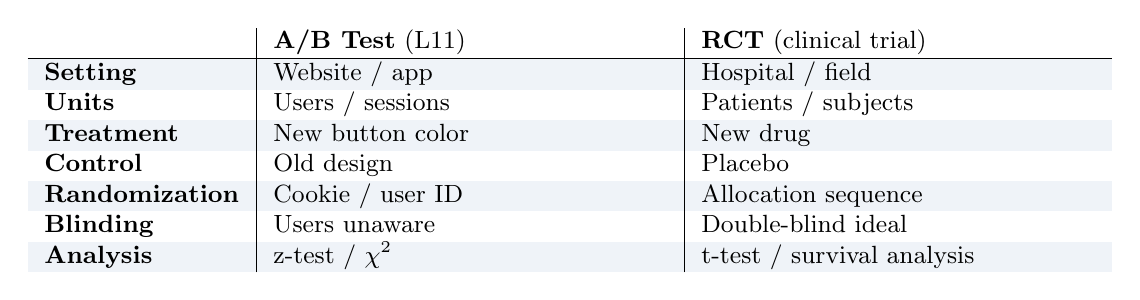
\begin{tikzpicture}
  \node[inner sep=0pt] {
    \small
    \begin{tabular}{l|p{5cm}|p{5cm}}
      & \textbf{A/B Test} (L11) & \textbf{RCT} (clinical trial) \\
      \hline
      \rowcolor{popblue!8}
      \textbf{Setting} & Website / app & Hospital / field \\
      \textbf{Units} & Users / sessions & Patients / subjects \\
      \rowcolor{popblue!8}
      \textbf{Treatment} & New button color & New drug \\
      \textbf{Control} & Old design & Placebo \\
      \rowcolor{popblue!8}
      \textbf{Randomization} & Cookie / user ID & Allocation sequence \\
      \textbf{Blinding} & Users unaware & Double-blind ideal \\
      \rowcolor{popblue!8}
      \textbf{Analysis} & z-test / $\chi^2$ & t-test / survival analysis \\
    \end{tabular}
  };
\end{tikzpicture}
\end{center}

\vspace{0.2cm}
\begin{center}
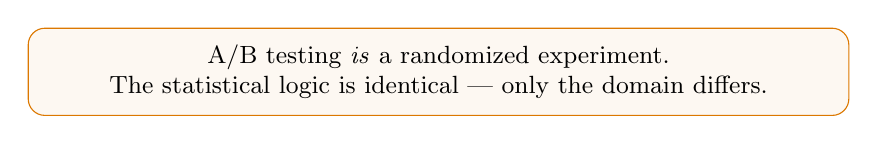
\begin{tikzpicture}
  \node[draw=orange1, fill=orange1!5, rounded corners=6pt, text width=10cm, align=center, inner sep=6pt, font=\small] {
    A/B testing \textit{is} a randomized experiment.\\
    The statistical logic is identical --- only the domain differs.
  };
\end{tikzpicture}
\end{center}
\end{frame}

% ============================================================
% PART III: POTENTIAL OUTCOMES
% ============================================================
\section{Potential Outcomes Framework}

\begin{frame}
\begin{center}
  \vspace{1.5cm}
  {\Huge\bfseries\textcolor{popblue}{Part III: Potential Outcomes}}

  \vspace{0.8cm}
  {\large The Rubin causal model}
\end{center}
\end{frame}

\begin{frame}
\frametitle{The Fundamental Problem of Causal Inference}

\begin{center}
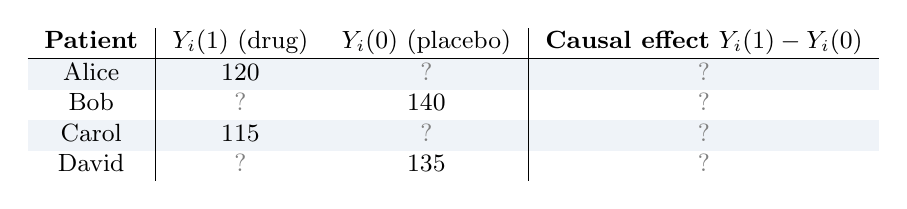
\begin{tikzpicture}
  \node[inner sep=0pt] {
    \small
    \begin{tabular}{c|cc|c}
      \textbf{Patient} & $Y_i(1)$ (drug) & $Y_i(0)$ (placebo) & \textbf{Causal effect} $Y_i(1) - Y_i(0)$ \\
      \hline
      \rowcolor{popblue!8}
      Alice & 120 & \textcolor{gray}{?} & \textcolor{gray}{?} \\
      Bob & \textcolor{gray}{?} & 140 & \textcolor{gray}{?} \\
      \rowcolor{popblue!8}
      Carol & 115 & \textcolor{gray}{?} & \textcolor{gray}{?} \\
      David & \textcolor{gray}{?} & 135 & \textcolor{gray}{?} \\
    \end{tabular}
  };
\end{tikzpicture}
\end{center}

\vspace{0.2cm}
\begin{center}
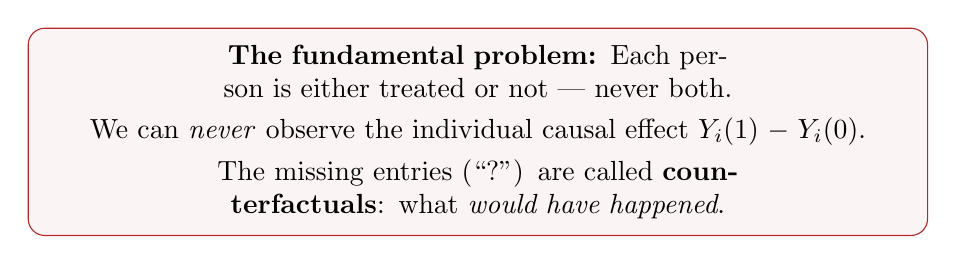
\begin{tikzpicture}
  \node[draw=warnred, fill=warnred!5, rounded corners=6pt, text width=11cm, align=center, inner sep=6pt] {
    \textbf{The fundamental problem:} Each person is either treated or not --- never both.\\[3pt]
    We can \textit{never} observe the individual causal effect $Y_i(1) - Y_i(0)$.\\[3pt]
    The missing entries (``?'') are called \textbf{counterfactuals}: what \textit{would have happened}.
  };
\end{tikzpicture}
\end{center}

\vspace{0.1cm}
\begin{center}

\begin{tikzpicture}
  \node[draw=popblue, fill=popblue!5, rounded corners=5pt, text width=10cm, align=center, inner sep=5pt, font=\small] {
    \textbf{Notation:} $Y_i(1)$ = outcome under treatment,
    $Y_i(0)$ = outcome under control. Only one is observed.
  };
\end{tikzpicture}
\end{center}
\end{frame}

\begin{frame}
\frametitle{Average Treatment Effect (ATE)}

\begin{center}
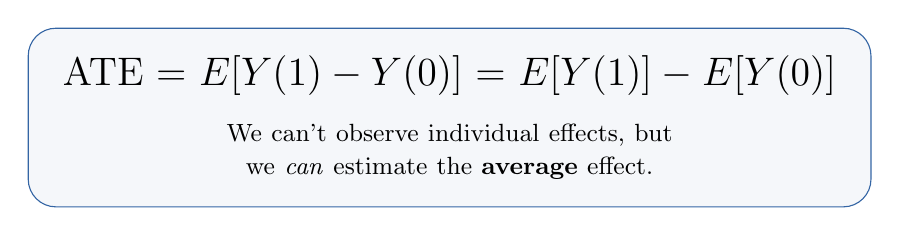
\begin{tikzpicture}
  \node[draw=popblue, fill=popblue!5, rounded corners=10pt, text width=10cm, align=center, inner sep=10pt] {
    {\Large $\text{ATE} = E\!\left[Y(1) - Y(0)\right] = E[Y(1)] - E[Y(0)]$}\\[8pt]
    \small We can't observe individual effects, but we \textit{can} estimate the \textbf{average} effect.
  };
\end{tikzpicture}
\end{center}

\vspace{0.3cm}
\begin{center}
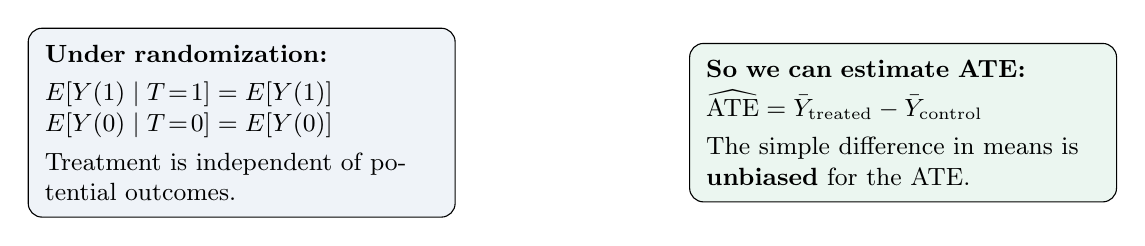
\begin{tikzpicture}[
  abox/.style={draw, rounded corners=5pt, text width=5cm, align=left, inner sep=6pt, font=\small}
]
  \node[abox, fill=popblue!8] at (-4.2, 0) {
    \textbf{Under randomization:}\\[3pt]
    $E[Y(1) \mid T\!=\!1] = E[Y(1)]$\\
    $E[Y(0) \mid T\!=\!0] = E[Y(0)]$\\[3pt]
    Treatment is independent of potential outcomes.
  };
  \node[abox, fill=paramgreen!8] at (4.2, 0) {
    \textbf{So we can estimate ATE:}\\[3pt]
    $\widehat{\text{ATE}} = \bar{Y}_\text{treated} - \bar{Y}_\text{control}$\\[3pt]
    The simple difference in means is \textbf{unbiased} for the ATE.
  };
\end{tikzpicture}
\end{center}

\vspace{0.2cm}
\begin{center}
\small\textcolor{gray}{Other estimands: ATT (on the treated), CATE (conditional), LATE (local) --- beyond our scope.}
\end{center}
\end{frame}

\begin{frame}
\frametitle{Why Randomization Identifies ATE}

\begin{center}
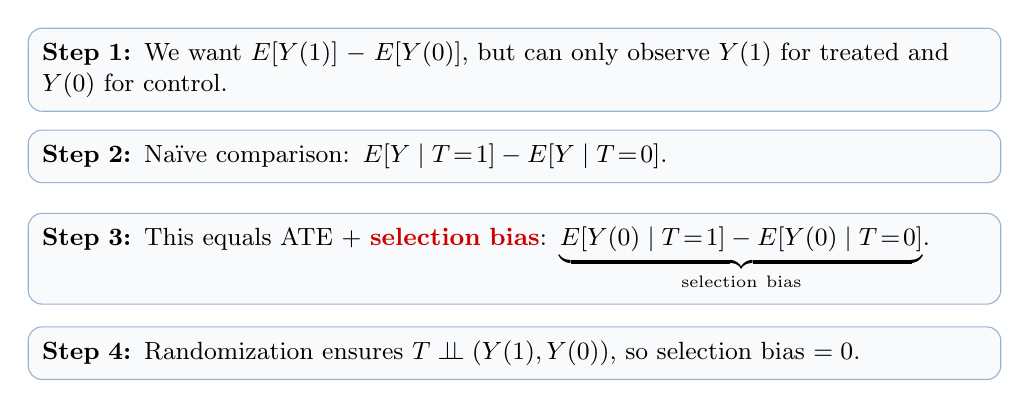
\begin{tikzpicture}[
  sbox/.style={draw=popblue!50, fill=popblue!3, rounded corners=5pt, text width=12cm, align=left, inner sep=5pt, font=\small}
]
  \node[sbox] at (0, 2.4) {
    \textbf{Step 1:} We want $E[Y(1)] - E[Y(0)]$, but can only observe $Y(1)$ for treated and $Y(0)$ for control.
  };
  \node[sbox] at (0, 1.3) {
    \textbf{Step 2:} Na\"ive comparison: $E[Y \mid T\!=\!1] - E[Y \mid T\!=\!0]$.
  };
  \node[sbox] at (0, 0.0) {
    \textbf{Step 3:} This equals ATE $+$ \textcolor{sampred}{\textbf{selection bias}}: $\underbrace{E[Y(0) \mid T\!=\!1] - E[Y(0) \mid T\!=\!0]}_{\text{selection bias}}$.
  };
  \node[sbox] at (0, -1.2) {
    \textbf{Step 4:} Randomization ensures $T \perp\!\!\!\perp (Y(1), Y(0))$, so selection bias $= 0$.
  };
\end{tikzpicture}
\end{center}

\vspace{0.1cm}
\begin{center}
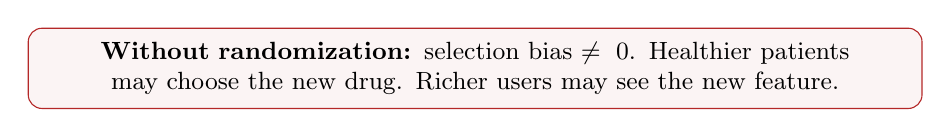
\begin{tikzpicture}
  \node[draw=warnred, fill=warnred!5, rounded corners=5pt, text width=11cm, align=center, inner sep=5pt, font=\small] {
    \textbf{Without randomization:} selection bias $\neq 0$.
    Healthier patients may choose the new drug. Richer users may see the new feature.
  };
\end{tikzpicture}
\end{center}
\end{frame}

% ============================================================
% PART IV: DAGs
% ============================================================
\section{Causal Graphs (DAGs)}

\begin{frame}
\begin{center}
  \vspace{1.5cm}
  {\Huge\bfseries\textcolor{popblue}{Part IV: Causal Graphs}}

  \vspace{0.8cm}
  {\large DAGs: seeing the causal structure}
\end{center}
\end{frame}

\begin{frame}
\frametitle{Directed Acyclic Graphs (DAGs)}

\begin{center}
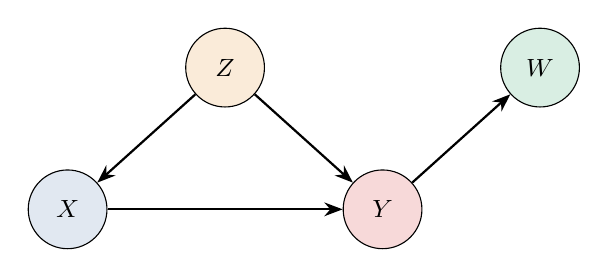
\begin{tikzpicture}[
  dnode/.style={draw, circle, minimum size=1cm, inner sep=0pt, font=\small\bfseries},
  arr/.style={-{Stealth}, thick}
]
  % Simple DAG
  \node[dnode, fill=popblue!15] (X) at (0, 0) {$X$};
  \node[dnode, fill=sampred!15] (Y) at (4, 0) {$Y$};
  \node[dnode, fill=orange1!15] (Z) at (2, 1.8) {$Z$};
  \node[dnode, fill=paramgreen!15] (W) at (6, 1.8) {$W$};

  \draw[arr] (Z) -- (X);
  \draw[arr] (Z) -- (Y);
  \draw[arr] (X) -- (Y);
  \draw[arr] (Y) -- (W);
\end{tikzpicture}
\end{center}

\vspace{0.2cm}
\begin{center}
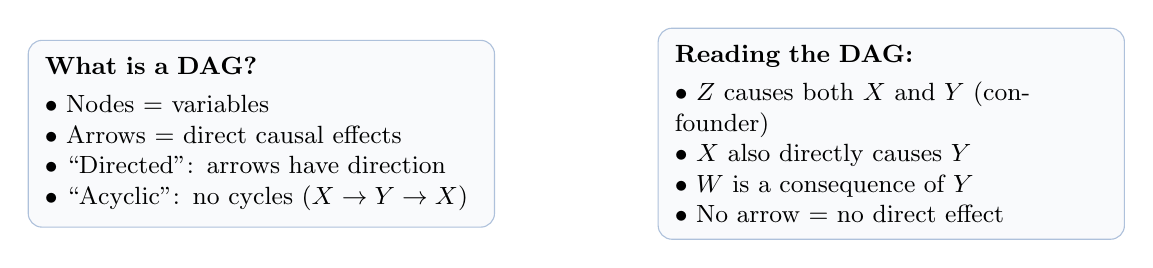
\begin{tikzpicture}[
  rbox/.style={draw=popblue!40, fill=popblue!3, rounded corners=5pt, text width=5.5cm, align=left, inner sep=6pt, font=\small}
]
  \node[rbox] at (-4, 0) {
    \textbf{What is a DAG?}\\[3pt]
    $\bullet$ Nodes = variables\\
    $\bullet$ Arrows = direct causal effects\\
    $\bullet$ ``Directed'': arrows have direction\\
    $\bullet$ ``Acyclic'': no cycles ($X \to Y \to X$)
  };
  \node[rbox] at (4, 0) {
    \textbf{Reading the DAG:}\\[3pt]
    $\bullet$ $Z$ causes both $X$ and $Y$ (confounder)\\
    $\bullet$ $X$ also directly causes $Y$\\
    $\bullet$ $W$ is a consequence of $Y$\\
    $\bullet$ No arrow = no direct effect
  };
\end{tikzpicture}
\end{center}
\end{frame}

\begin{frame}
\frametitle{Three Fundamental Structures}

\begin{center}
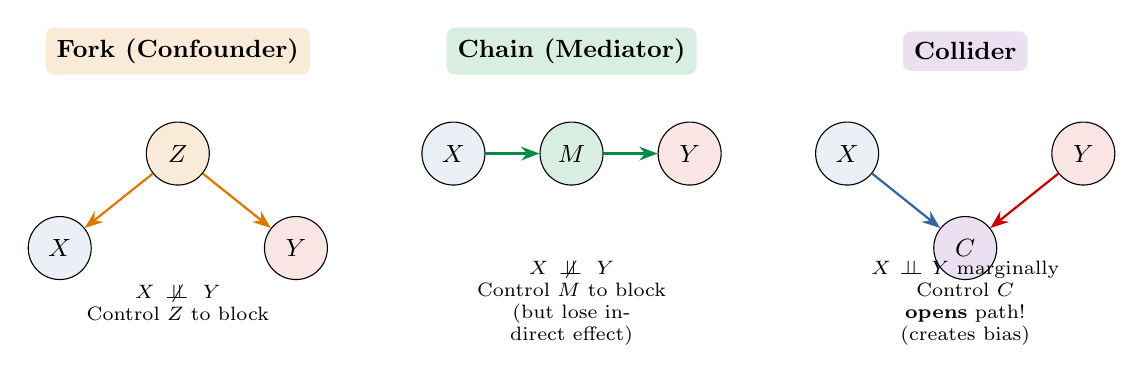
\begin{tikzpicture}[
  dnode/.style={draw, circle, minimum size=0.8cm, inner sep=0pt, font=\small\bfseries},
  arr/.style={-{Stealth}, thick},
  lbl/.style={font=\small\bfseries}
]
  % --- Fork (confounder) ---
  \node[lbl, fill=orange1!15, rounded corners=3pt, inner sep=4pt] at (-5, 2.5) {Fork (Confounder)};
  \node[dnode, fill=orange1!15] (fz) at (-5, 1.2) {$Z$};
  \node[dnode, fill=popblue!10] (fx) at (-6.5, 0) {$X$};
  \node[dnode, fill=sampred!10] (fy) at (-3.5, 0) {$Y$};
  \draw[arr, orange1] (fz) -- (fx);
  \draw[arr, orange1] (fz) -- (fy);
  \node[font=\scriptsize, text width=2.5cm, align=center] at (-5, -0.7) {$X \not\!\perp\!\!\!\perp Y$\\Control $Z$ to block};

  % --- Chain (mediator) ---
  \node[lbl, fill=paramgreen!15, rounded corners=3pt, inner sep=4pt] at (0, 2.5) {Chain (Mediator)};
  \node[dnode, fill=popblue!10] (cx) at (-1.5, 1.2) {$X$};
  \node[dnode, fill=paramgreen!15] (cm) at (0, 1.2) {$M$};
  \node[dnode, fill=sampred!10] (cy) at (1.5, 1.2) {$Y$};
  \draw[arr, paramgreen] (cx) -- (cm);
  \draw[arr, paramgreen] (cm) -- (cy);
  \node[font=\scriptsize, text width=2.5cm, align=center] at (0, -0.7) {$X \not\!\perp\!\!\!\perp Y$\\Control $M$ to block\\(but lose indirect effect)};

  % --- Collider ---
  \node[lbl, fill=violet1!15, rounded corners=3pt, inner sep=4pt] at (5, 2.5) {Collider};
  \node[dnode, fill=popblue!10] (lx) at (3.5, 1.2) {$X$};
  \node[dnode, fill=sampred!10] (ly) at (6.5, 1.2) {$Y$};
  \node[dnode, fill=violet1!15] (lc) at (5, 0) {$C$};
  \draw[arr, popblue] (lx) -- (lc);
  \draw[arr, sampred] (ly) -- (lc);
  \node[font=\scriptsize, text width=2.8cm, align=center] at (5, -0.7) {$X \perp\!\!\!\perp Y$ marginally\\Control $C$ \textbf{opens} path!\\(creates bias)};
\end{tikzpicture}
\end{center}

\vspace{0.2cm}
\begin{center}

\begin{tikzpicture}
  \node[draw=warnred, fill=warnred!5, rounded corners=6pt, text width=11cm, align=center, inner sep=6pt, font=\small] {
    \textbf{Key insight:} Conditioning on a confounder \textit{removes} bias. Conditioning on a collider \textit{creates} bias.\\
    You must know the DAG to decide what to control for.
  };
\end{tikzpicture}
\end{center}
\end{frame}

\begin{frame}
\frametitle{Collider Bias: A Concrete Example}
\framesubtitle{The ``talent vs attractiveness'' paradox}

\begin{center}
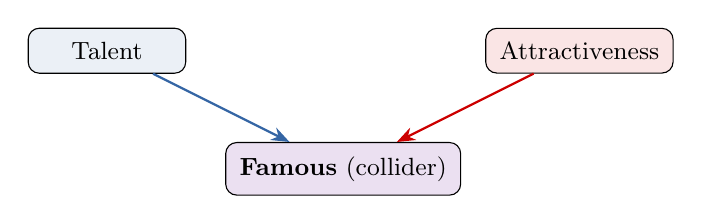
\begin{tikzpicture}[
  dnode/.style={draw, rounded corners=4pt, inner sep=5pt, font=\small, minimum width=2cm, align=center},
  arr/.style={-{Stealth}, thick}
]
  \node[dnode, fill=popblue!10] (T) at (-3, 1.5) {Talent};
  \node[dnode, fill=sampred!10] (A) at (3, 1.5) {Attractiveness};
  \node[dnode, fill=violet1!15] (F) at (0, 0) {\textbf{Famous} (collider)};

  \draw[arr, popblue] (T) -- (F);
  \draw[arr, sampred] (A) -- (F);
\end{tikzpicture}
\end{center}

\vspace{0.2cm}
\begin{center}
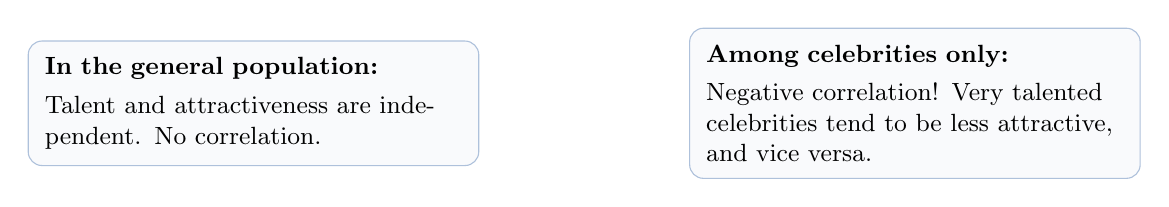
\begin{tikzpicture}[
  ebox/.style={draw=popblue!40, fill=popblue!3, rounded corners=5pt, text width=5.3cm, align=left, inner sep=6pt, font=\small}
]
  \node[ebox] at (-4.2, 0) {
    \textbf{In the general population:}\\[3pt]
    Talent and attractiveness are independent. No correlation.
  };
  \node[ebox] at (4.2, 0) {
    \textbf{Among celebrities only:}\\[3pt]
    Negative correlation! Very talented celebrities tend to be less attractive, and vice versa.
  };
\end{tikzpicture}
\end{center}

\vspace{0.1cm}
\begin{center}
\small By conditioning on the collider (``among the famous''), we \textit{created} a spurious association.\\
\textcolor{gray}{Same logic: ``Why are all my dates either boring or unstable?'' --- you're conditioning on ``agreed to date me.''}
\end{center}
\end{frame}

\begin{frame}
\frametitle{Simpson's Paradox Revisited}
\framesubtitle{From L2 --- now we have the language to explain it}

\begin{center}
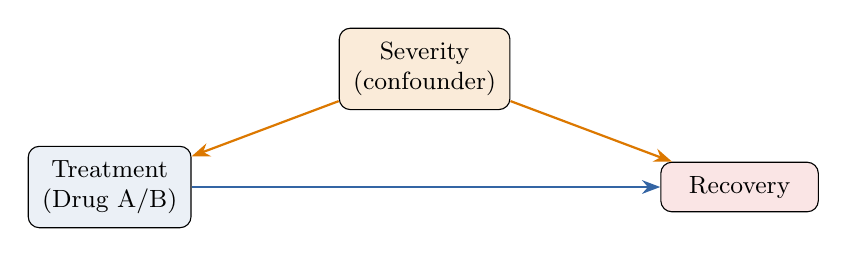
\begin{tikzpicture}[
  dnode/.style={draw, rounded corners=4pt, inner sep=5pt, font=\small, minimum width=2cm, align=center},
  arr/.style={-{Stealth}, thick}
]
  \node[dnode, fill=popblue!10] (T) at (-4, 0) {Treatment\\(Drug A/B)};
  \node[dnode, fill=orange1!15] (S) at (0, 1.5) {Severity\\(confounder)};
  \node[dnode, fill=sampred!10] (Y) at (4, 0) {Recovery};

  \draw[arr, popblue] (T) -- (Y);
  \draw[arr, orange1] (S) -- (T);
  \draw[arr, orange1] (S) -- (Y);
\end{tikzpicture}
\end{center}

\vspace{0.2cm}
\begin{center}
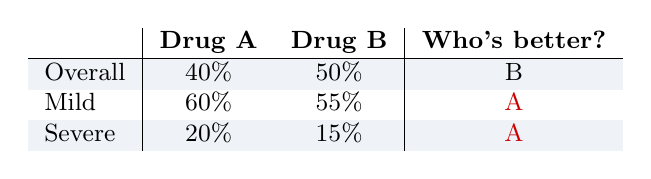
\begin{tikzpicture}
  \node[inner sep=0pt] {
    \small
    \begin{tabular}{l|cc|c}
      & \textbf{Drug A} & \textbf{Drug B} & \textbf{Who's better?} \\
      \hline
      \rowcolor{popblue!8}
      Overall & 40\% & 50\% & B \\
      Mild & 60\% & 55\% & \textcolor{sampred}{A} \\
      \rowcolor{popblue!8}
      Severe & 20\% & 15\% & \textcolor{sampred}{A} \\
    \end{tabular}
  };
\end{tikzpicture}
\end{center}

\vspace{0.1cm}
\begin{center}
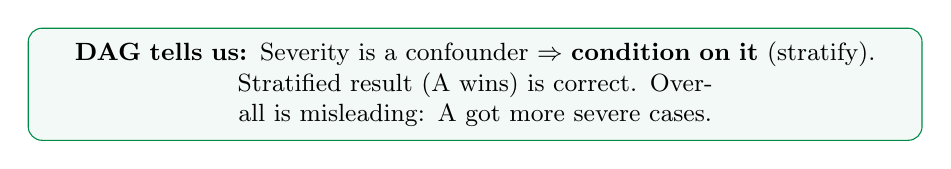
\begin{tikzpicture}
  \node[draw=paramgreen, fill=paramgreen!5, rounded corners=5pt, text width=11cm, align=center, inner sep=5pt, font=\small] {
    \textbf{DAG tells us:} Severity is a confounder $\Rightarrow$ \textbf{condition on it} (stratify).\\
    Stratified result (A wins) is correct. Overall is misleading: A got more severe cases.
  };
\end{tikzpicture}
\end{center}
\end{frame}

% ============================================================
% PART V: OBSERVATIONAL STUDIES
% ============================================================
\section{Observational Studies}

\begin{frame}
\begin{center}
  \vspace{1.5cm}
  {\Huge\bfseries\textcolor{popblue}{Part V: When You Can't Randomize}}

  \vspace{0.8cm}
  {\large Observational causal inference}
\end{center}
\end{frame}

\begin{frame}
\frametitle{The Problem with Observational Data}

\begin{center}
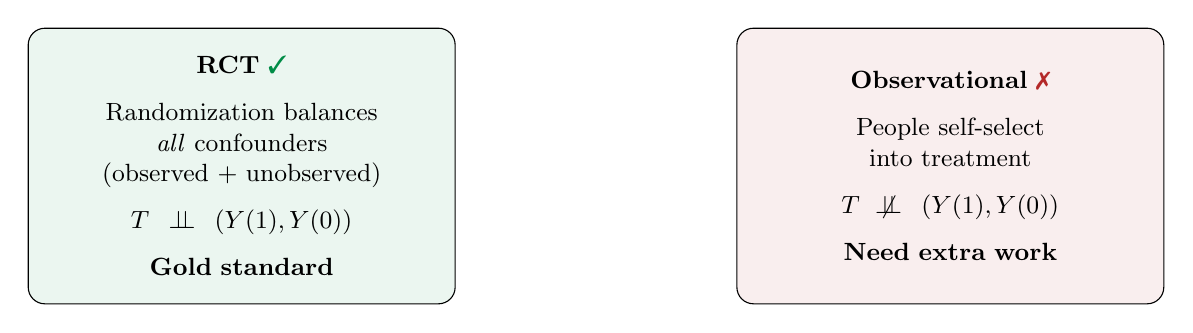
\begin{tikzpicture}[
  cbox/.style={draw, rounded corners=6pt, text width=5cm, align=center, inner sep=6pt, font=\small, minimum height=3.5cm}
]
  \node[cbox, fill=paramgreen!8] at (-4.5, 0) {
    \textbf{RCT} \textcolor{paramgreen}{\ding{51}}\\[6pt]
    Randomization balances\\
    \textit{all} confounders\\
    (observed + unobserved)\\[6pt]
    $T \perp\!\!\!\perp (Y(1), Y(0))$\\[6pt]
    \textbf{Gold standard}
  };
  \node[cbox, fill=warnred!8] at (4.5, 0) {
    \textbf{Observational} \textcolor{warnred}{\ding{55}}\\[6pt]
    People self-select\\
    into treatment\\[6pt]
    $T \not\!\perp\!\!\!\perp (Y(1), Y(0))$\\[6pt]
    \textbf{Need extra work}
  };
\end{tikzpicture}
\end{center}

\vspace{0.2cm}
\begin{center}
\small When can't we randomize? Ethics (can't assign smoking), cost, logistics, already-collected data.\\
We need methods that approximate what randomization does.
\end{center}
\end{frame}

\begin{frame}
\frametitle{Strategy 1: Conditioning / Regression}
\framesubtitle{Control for confounders directly}

\begin{center}
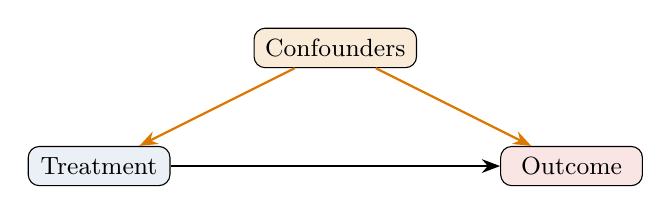
\begin{tikzpicture}[
  dnode/.style={draw, rounded corners=4pt, inner sep=4pt, font=\small, minimum width=1.8cm, align=center},
  arr/.style={-{Stealth}, thick}
]
  \node[dnode, fill=popblue!10] (T) at (-3, 0) {Treatment};
  \node[dnode, fill=sampred!10] (Y) at (3, 0) {Outcome};
  \node[dnode, fill=orange1!15] (Z) at (0, 1.5) {Confounders};
  \draw[arr] (T) -- (Y);
  \draw[arr, orange1] (Z) -- (T);
  \draw[arr, orange1] (Z) -- (Y);
\end{tikzpicture}
\end{center}

\vspace{0.1cm}
\begin{center}
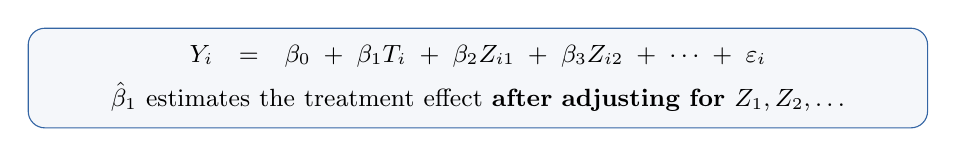
\begin{tikzpicture}
  \node[draw=popblue, fill=popblue!5, rounded corners=6pt, text width=11cm, align=center, inner sep=6pt] {
    {\small $Y_i = \beta_0 + \beta_1 T_i + \beta_2 Z_{i1} + \beta_3 Z_{i2} + \cdots + \varepsilon_i$}\\[4pt]
    \small $\hat\beta_1$ estimates the treatment effect \textbf{after adjusting for} $Z_1, Z_2, \ldots$
  };
\end{tikzpicture}
\end{center}

\vspace{0.2cm}
\begin{center}
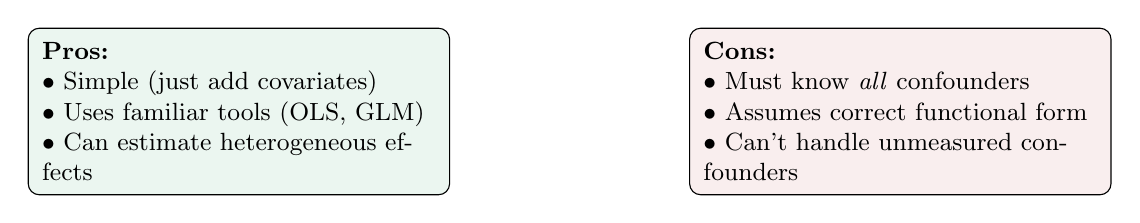
\begin{tikzpicture}[
  pbox/.style={draw, rounded corners=4pt, text width=5cm, align=left, inner sep=5pt, font=\small}
]
  \node[pbox, fill=paramgreen!8] at (-4.2, 0) {
    \textbf{Pros:}\\
    $\bullet$ Simple (just add covariates)\\
    $\bullet$ Uses familiar tools (OLS, GLM)\\
    $\bullet$ Can estimate heterogeneous effects
  };
  \node[pbox, fill=warnred!8] at (4.2, 0) {
    \textbf{Cons:}\\
    $\bullet$ Must know \textit{all} confounders\\
    $\bullet$ Assumes correct functional form\\
    $\bullet$ Can't handle unmeasured confounders
  };
\end{tikzpicture}
\end{center}
\end{frame}

\begin{frame}
\frametitle{Strategy 2: Matching}
\framesubtitle{Find ``twins'' --- one treated, one not}

\begin{center}
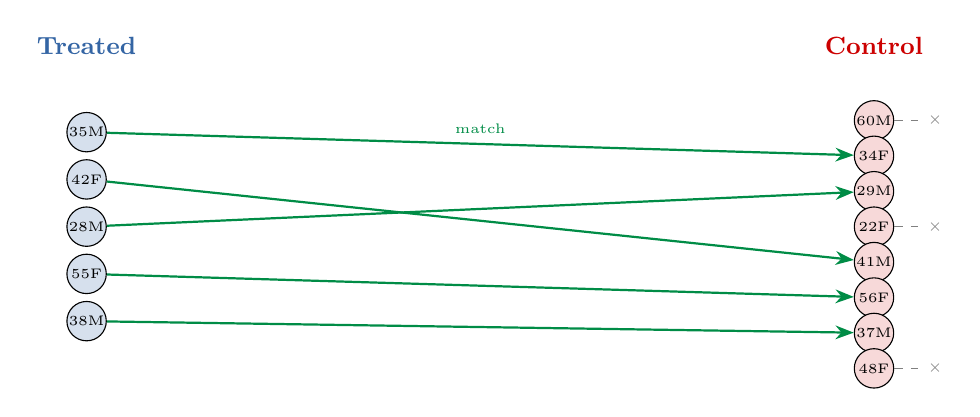
\begin{tikzpicture}[
  person/.style={draw, circle, minimum size=0.5cm, inner sep=0pt, font=\tiny}
]
  % Treated
  \node[font=\small\bfseries, popblue] at (-5, 2.0) {Treated};
  \foreach \i/\a/\s in {1/35/M, 2/42/F, 3/28/M, 4/55/F, 5/38/M} {
    \node[person, fill=popblue!20] (t\i) at (-5, 1.5 - \i*0.6) {\a\s};
  }

  % Control
  \node[font=\small\bfseries, sampred] at (5, 2.0) {Control};
  \foreach \i/\a/\s in {1/60/M, 2/34/F, 3/29/M, 4/22/F, 5/41/M, 6/56/F, 7/37/M, 8/48/F} {
    \node[person, fill=sampred!15] (c\i) at (5, 1.5 - \i*0.45) {\a\s};
  }

  % Matches
  \draw[thick, paramgreen, -{Stealth}] (t1) -- (c2) node[midway, above, font=\tiny, paramgreen] {match};
  \draw[thick, paramgreen, -{Stealth}] (t2) -- (c5);
  \draw[thick, paramgreen, -{Stealth}] (t3) -- (c3);
  \draw[thick, paramgreen, -{Stealth}] (t4) -- (c6);
  \draw[thick, paramgreen, -{Stealth}] (t5) -- (c7);

  % Unmatched
  \draw[gray, dashed] (c1.east) -- ++(0.3, 0) node[right, font=\tiny, gray] {$\times$};
  \draw[gray, dashed] (c4.east) -- ++(0.3, 0) node[right, font=\tiny, gray] {$\times$};
  \draw[gray, dashed] (c8.east) -- ++(0.3, 0) node[right, font=\tiny, gray] {$\times$};
\end{tikzpicture}
\end{center}

\vspace{0.05cm}
\begin{center}

\begin{tikzpicture}
  \node[draw=paramgreen, fill=paramgreen!5, rounded corners=5pt, text width=11cm, align=center, inner sep=5pt, font=\small] {
    For each treated unit, find a control with \textbf{similar covariates} (age, sex, \ldots).
    Compare outcomes within matched pairs. Unmatched controls are discarded.
  };
\end{tikzpicture}
\end{center}
\end{frame}

\begin{frame}
\frametitle{Strategy 3: Propensity Score}
\framesubtitle{Rosenbaum \& Rubin (1983)}

\begin{center}
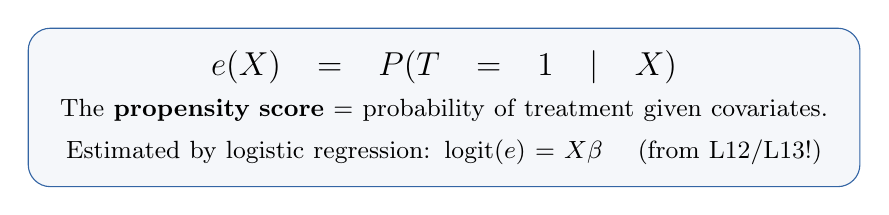
\begin{tikzpicture}
  \node[draw=popblue, fill=popblue!5, rounded corners=8pt, text width=10cm, align=center, inner sep=8pt] {
    {\large $e(X) = P(T = 1 \mid X)$}\\[4pt]
    \small The \textbf{propensity score} = probability of treatment given covariates.\\[3pt]
    Estimated by logistic regression: $\text{logit}(e) = X\beta$ \quad(from L12/L13!)
  };
\end{tikzpicture}
\end{center}

\vspace{0.1cm}
\begin{center}
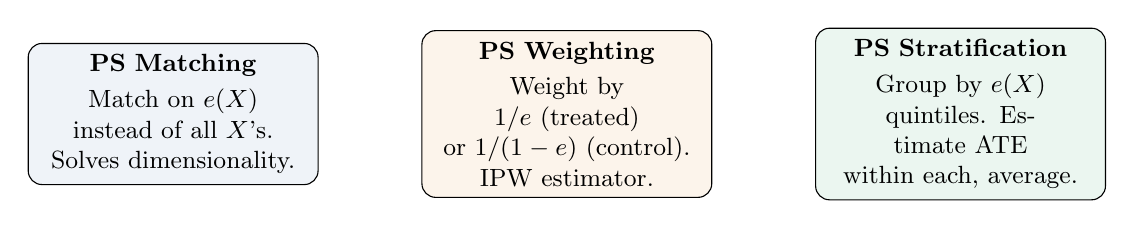
\begin{tikzpicture}[
  mbox/.style={draw, rounded corners=5pt, text width=3.4cm, align=center, inner sep=4pt, font=\small, minimum height=1.6cm}
]
  \node[mbox, fill=popblue!8] at (-5, 0) {
    \textbf{PS Matching}\\[2pt]
    Match on $e(X)$\\instead of all $X$'s.\\
    Solves dimensionality.
  };
  \node[mbox, fill=orange1!8] at (0, 0) {
    \textbf{PS Weighting}\\[2pt]
    Weight by $1/e$ (treated)\\or $1/(1-e)$ (control).\\
    IPW estimator.
  };
  \node[mbox, fill=paramgreen!8] at (5, 0) {
    \textbf{PS Stratification}\\[2pt]
    Group by $e(X)$\\quintiles. Estimate ATE\\within each, average.
  };
\end{tikzpicture}
\end{center}

\vspace{0.1cm}
\begin{center}
\small\textbf{Key theorem:} If treatment is ignorable given $X$, it's also ignorable given $e(X)$ alone.
\end{center}
\end{frame}

\begin{frame}
\frametitle{Strategy 4: Instrumental Variables}
\framesubtitle{When you can't measure all confounders}

\begin{center}
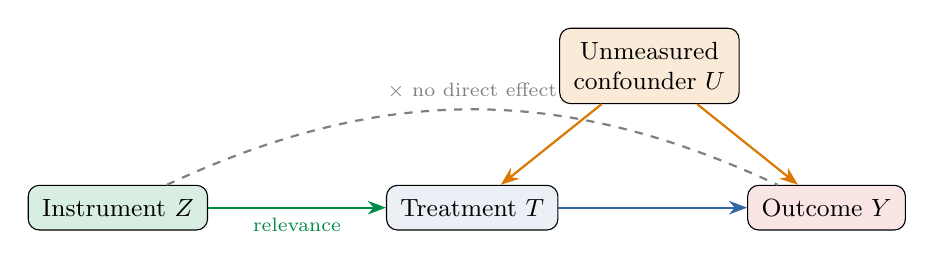
\begin{tikzpicture}[
  dnode/.style={draw, rounded corners=4pt, inner sep=5pt, font=\small, minimum width=2cm, align=center},
  arr/.style={-{Stealth}, thick}
]
  \node[dnode, fill=paramgreen!15] (Z) at (-4.5, 0) {Instrument $Z$};
  \node[dnode, fill=popblue!10] (T) at (0, 0) {Treatment $T$};
  \node[dnode, fill=sampred!10] (Y) at (4.5, 0) {Outcome $Y$};
  \node[dnode, fill=orange1!15] (U) at (2.25, 1.8) {Unmeasured\\confounder $U$};

  \draw[arr, paramgreen] (Z) -- (T) node[midway, below, font=\scriptsize] {relevance};
  \draw[arr, popblue] (T) -- (Y);
  \draw[arr, orange1] (U) -- (T);
  \draw[arr, orange1] (U) -- (Y);

  % No direct effect
  \draw[dashed, gray, thick] (Z) to[bend left=25] node[midway, above, font=\scriptsize, gray] {$\times$ no direct effect} (Y);
\end{tikzpicture}
\end{center}

\vspace{0.2cm}
\begin{center}
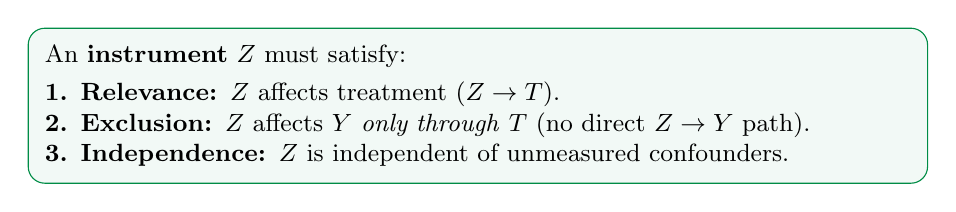
\begin{tikzpicture}
  \node[draw=paramgreen, fill=paramgreen!5, rounded corners=6pt, text width=11cm, align=left, inner sep=6pt, font=\small] {
    An \textbf{instrument} $Z$ must satisfy:\\[3pt]
    \textbf{1. Relevance:} $Z$ affects treatment ($Z \to T$).\\
    \textbf{2. Exclusion:} $Z$ affects $Y$ \textit{only through} $T$ (no direct $Z \to Y$ path).\\
    \textbf{3. Independence:} $Z$ is independent of unmeasured confounders.
  };
\end{tikzpicture}
\end{center}

\vspace{0.1cm}
\begin{center}
\small\textbf{Example:} Effect of military service on earnings.
Instrument: draft lottery number (random, affects service, no direct effect on earnings).
\end{center}
\end{frame}

% ============================================================
% PART VI: DO vs SEE
% ============================================================
\section{Doing vs Seeing}

\begin{frame}
\begin{center}
  \vspace{1.5cm}
  {\Huge\bfseries\textcolor{popblue}{Part VI: Doing $\neq$ Seeing}}

  \vspace{0.8cm}
  {\large $P(Y \mid X)$ vs $P(Y \mid \text{do}(X))$}
\end{center}
\end{frame}

\begin{frame}
\frametitle{Observing vs Intervening}

\begin{center}
\begin{tikzpicture}[
  cbox/.style={draw, rounded corners=5pt, text width=5.3cm, align=center, inner sep=5pt, font=\small, minimum height=3cm}
]
  \node[cbox, fill=popblue!8] at (-4.5, 0) {
    \textbf{Observing: $P(Y \mid X\!=\!x)$}\\[3pt]
    \begin{tikzpicture}[scale=0.5]
      \node[draw, circle, fill=orange1!15, inner sep=2pt, font=\scriptsize] (z) at (0,1.3) {$Z$};
      \node[draw, circle, fill=popblue!15, inner sep=2pt, font=\scriptsize] (x) at (-1.3,0) {$X$};
      \node[draw, circle, fill=sampred!15, inner sep=2pt, font=\scriptsize] (y) at (1.3,0) {$Y$};
      \draw[-{Stealth}, thick] (z) -- (x);
      \draw[-{Stealth}, thick] (z) -- (y);
      \draw[-{Stealth}, thick] (x) -- (y);
    \end{tikzpicture}\\[3pt]
    {\footnotesize ``What is $Y$ among those\\who \textit{happened to} take $X\!=\!x$?''}
  };
  \node[cbox, fill=paramgreen!8] at (4.5, 0) {
    \textbf{Intervening: $P(Y \mid \text{do}(X\!=\!x))$}\\[3pt]
    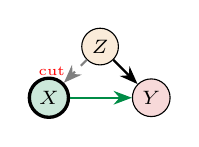
\begin{tikzpicture}[scale=0.5]
      \node[draw, circle, fill=orange1!15, inner sep=2pt, font=\scriptsize] (z) at (0,1.3) {$Z$};
      \node[draw, circle, fill=paramgreen!20, inner sep=2pt, font=\scriptsize, very thick] (x) at (-1.3,0) {$X$};
      \node[draw, circle, fill=sampred!15, inner sep=2pt, font=\scriptsize] (y) at (1.3,0) {$Y$};
      \draw[-{Stealth}, thick, gray, dashed] (z) -- (x) node[midway, left, font=\tiny, red] {cut};
      \draw[-{Stealth}, thick] (z) -- (y);
      \draw[-{Stealth}, thick, paramgreen] (x) -- (y);
    \end{tikzpicture}\\[3pt]
    {\footnotesize ``If we \textit{force} $X\!=\!x$,\\what is $Y$?'' Arrows into $X$ cut.}
  };
\end{tikzpicture}
\end{center}

\vspace{0.05cm}
\begin{center}
\small The $\text{do}(\cdot)$ operator (Pearl) formalizes intervention: set $X$ externally, severing all causes of $X$.
\end{center}
\end{frame}

\begin{frame}
\frametitle{The Backdoor Criterion}
\framesubtitle{When can we estimate causal effects from observational data?}

\begin{center}
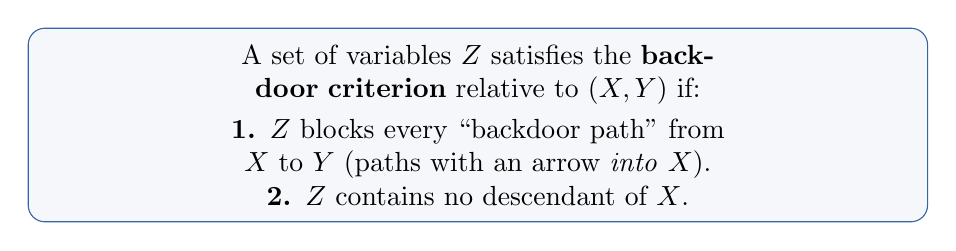
\begin{tikzpicture}
  \node[draw=popblue, fill=popblue!5, rounded corners=6pt, text width=11cm, align=center, inner sep=6pt] {
    A set of variables $Z$ satisfies the \textbf{backdoor criterion} relative to $(X, Y)$ if:\\[3pt]
    \textbf{1.} $Z$ blocks every ``backdoor path'' from $X$ to $Y$ (paths with an arrow \textit{into} $X$).\\
    \textbf{2.} $Z$ contains no descendant of $X$.
  };
\end{tikzpicture}
\end{center}

\vspace{0.1cm}
\begin{center}
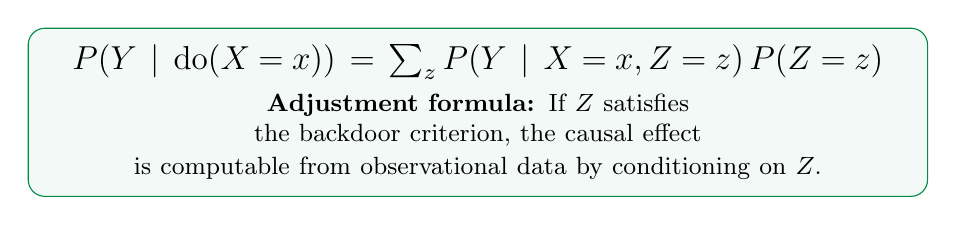
\begin{tikzpicture}
  \node[draw=paramgreen, fill=paramgreen!5, rounded corners=6pt, text width=11cm, align=center, inner sep=6pt] {
    {\large $P(Y \mid \text{do}(X\!=\!x)) = \sum_z P(Y \mid X\!=\!x, Z\!=\!z)\, P(Z\!=\!z)$}\\[4pt]
    \small \textbf{Adjustment formula:} If $Z$ satisfies the backdoor criterion, the causal effect\\
    is computable from observational data by conditioning on $Z$.
  };
\end{tikzpicture}
\end{center}

\vspace{0.1cm}
\begin{center}
\small This is exactly what regression does when you ``control for'' confounders. The DAG tells you \textit{which} variables to control for.
\end{center}
\end{frame}

% ============================================================
% PART VII: PRACTICAL CHECKLIST
% ============================================================
\section{Practical Causal Analysis}

\begin{frame}
\begin{center}
  \vspace{1.5cm}
  {\Huge\bfseries\textcolor{popblue}{Part VII: In Practice}}

  \vspace{0.8cm}
  {\large A checklist for causal claims}
\end{center}
\end{frame}

\begin{frame}
\frametitle{The Ladder of Causation}
\framesubtitle{Pearl's three levels}

\begin{center}
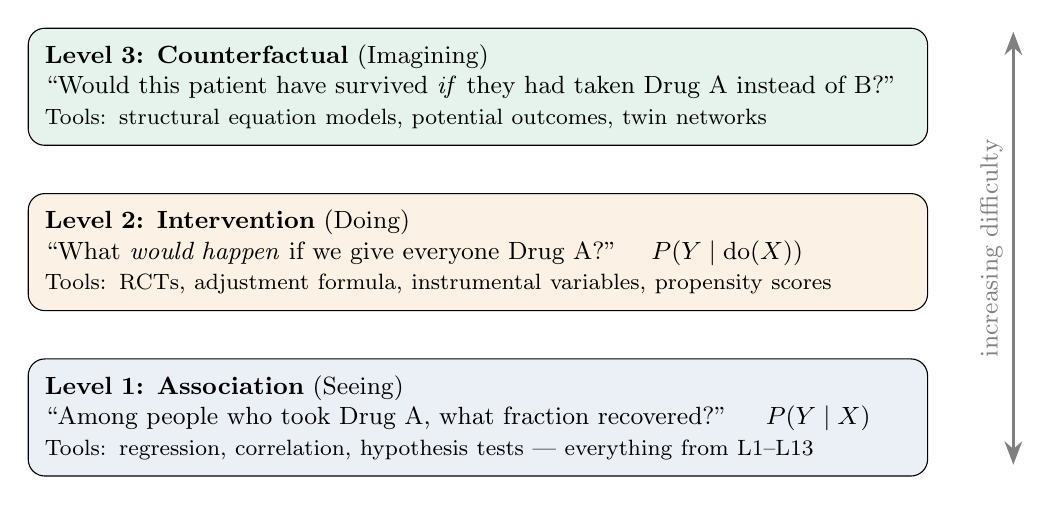
\begin{tikzpicture}[
  lbox/.style={draw, rounded corners=6pt, text width=11cm, align=left, inner sep=6pt, font=\small, minimum height=1.3cm}
]
  \node[lbox, fill=paramgreen!10] at (0, 3.0) {
    \textbf{Level 3: Counterfactual} (Imagining)\\
    ``Would this patient have survived \textit{if} they had taken Drug A instead of B?''\\
    {\footnotesize Tools: structural equation models, potential outcomes, twin networks}
  };
  \node[lbox, fill=orange1!10] at (0, 0.9) {
    \textbf{Level 2: Intervention} (Doing)\\
    ``What \textit{would happen} if we give everyone Drug A?'' \quad $P(Y \mid \text{do}(X))$\\
    {\footnotesize Tools: RCTs, adjustment formula, instrumental variables, propensity scores}
  };
  \node[lbox, fill=popblue!10] at (0, -1.2) {
    \textbf{Level 1: Association} (Seeing)\\
    ``Among people who took Drug A, what fraction recovered?'' \quad $P(Y \mid X)$\\
    {\footnotesize Tools: regression, correlation, hypothesis tests --- everything from L1--L13}
  };

  % Arrow
  \draw[{Stealth}-{Stealth}, very thick, gray] (6.8, -1.8) -- (6.8, 3.7) node[midway, right, font=\small, gray, rotate=90, anchor=south] {increasing difficulty};
\end{tikzpicture}
\end{center}
\end{frame}

\begin{frame}
\frametitle{Causal Inference Checklist}

\begin{center}
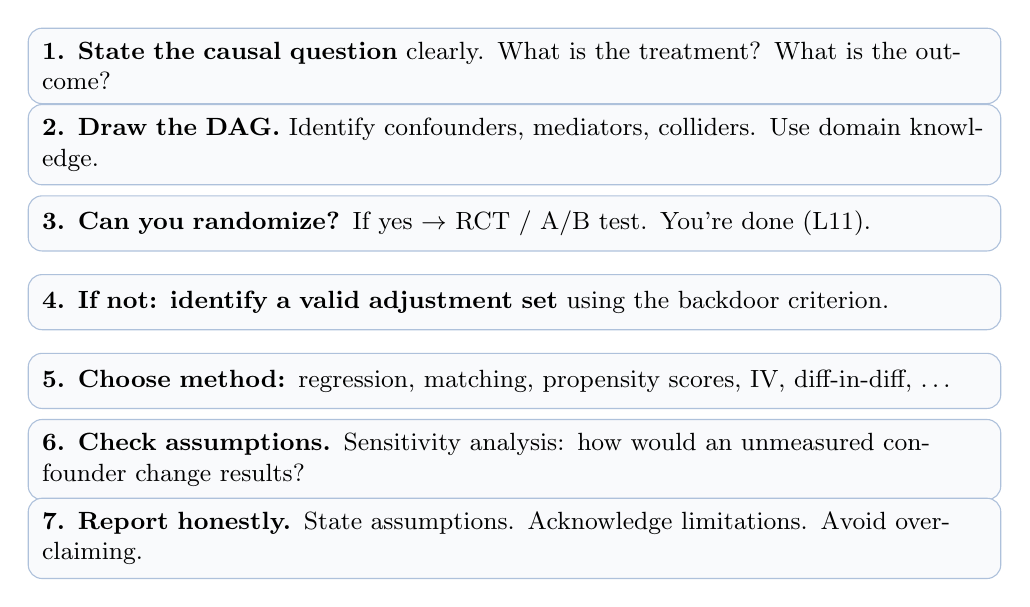
\begin{tikzpicture}[
  stp/.style={draw=popblue!40, fill=popblue!3, rounded corners=5pt, text width=12cm, align=left, inner sep=5pt, font=\small, minimum height=0.7cm}
]
  \node[stp] at (0, 3.2) {\textbf{1. State the causal question} clearly. What is the treatment? What is the outcome?};
  \node[stp] at (0, 2.2) {\textbf{2. Draw the DAG.} Identify confounders, mediators, colliders. Use domain knowledge.};
  \node[stp] at (0, 1.2) {\textbf{3. Can you randomize?} If yes $\to$ RCT / A/B test. You're done (L11).};
  \node[stp] at (0, 0.2) {\textbf{4. If not: identify a valid adjustment set} using the backdoor criterion.};
  \node[stp] at (0, -0.8) {\textbf{5. Choose method:} regression, matching, propensity scores, IV, diff-in-diff, \ldots};
  \node[stp] at (0, -1.8) {\textbf{6. Check assumptions.} Sensitivity analysis: how would an unmeasured confounder change results?};
  \node[stp] at (0, -2.8) {\textbf{7. Report honestly.} State assumptions. Acknowledge limitations. Avoid overclaiming.};
\end{tikzpicture}
\end{center}
\end{frame}

\begin{frame}
\frametitle{Common Pitfalls}

\begin{center}
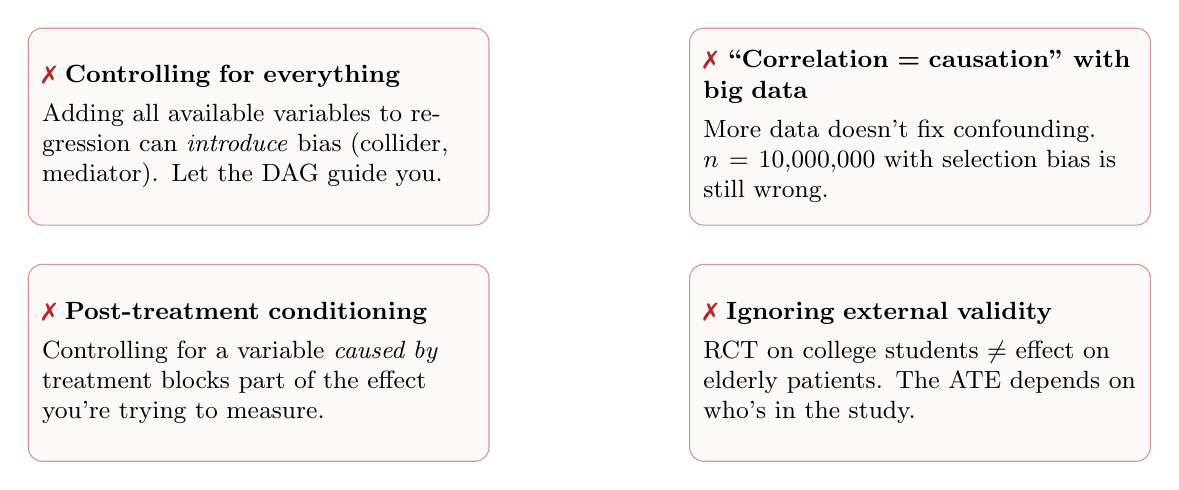
\begin{tikzpicture}[
  pbox/.style={draw=warnred!50, fill=warnred!3, rounded corners=5pt, text width=5.5cm, align=left, inner sep=5pt, font=\small, minimum height=2.5cm}
]
  \node[pbox] at (-4.2, 1.5) {
    \textbf{\textcolor{warnred}{\ding{55}} Controlling for everything}\\[3pt]
    Adding all available variables to regression can \textit{introduce} bias (collider, mediator). Let the DAG guide you.
  };
  \node[pbox] at (4.2, 1.5) {
    \textbf{\textcolor{warnred}{\ding{55}} ``Correlation = causation'' with big data}\\[3pt]
    More data doesn't fix confounding. $n = 10{,}000{,}000$ with selection bias is still wrong.
  };
  \node[pbox] at (-4.2, -1.5) {
    \textbf{\textcolor{warnred}{\ding{55}} Post-treatment conditioning}\\[3pt]
    Controlling for a variable \textit{caused by} treatment blocks part of the effect you're trying to measure.
  };
  \node[pbox] at (4.2, -1.5) {
    \textbf{\textcolor{warnred}{\ding{55}} Ignoring external validity}\\[3pt]
    RCT on college students $\neq$ effect on elderly patients. The ATE depends on who's in the study.
  };
\end{tikzpicture}
\end{center}
\end{frame}

% ============================================================
% SUMMARY
% ============================================================
\section*{Summary}

\begin{frame}
\frametitle{Summary: Causal Inference}

\begin{center}
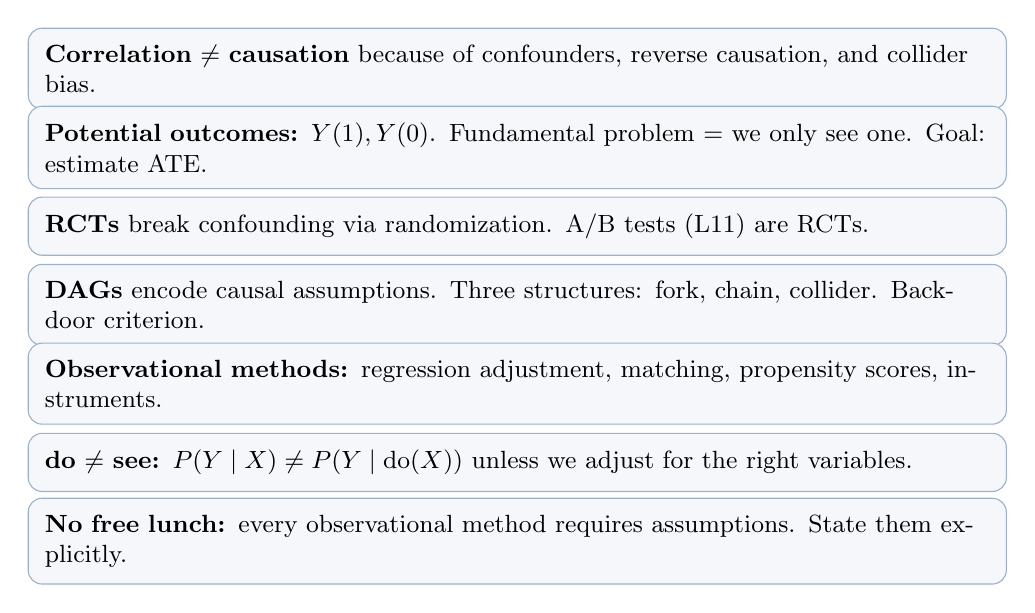
\begin{tikzpicture}[
  sbox/.style={draw=popblue!50, fill=popblue!5, rounded corners=5pt, text width=12cm, align=left, inner sep=6pt, font=\small}
]
  \node[sbox] at (0, 3.0) {
    \textbf{Correlation $\neq$ causation} because of confounders, reverse causation, and collider bias.
  };
  \node[sbox] at (0, 2.0) {
    \textbf{Potential outcomes:} $Y(1), Y(0)$. Fundamental problem = we only see one. Goal: estimate ATE.
  };
  \node[sbox] at (0, 1.0) {
    \textbf{RCTs} break confounding via randomization. A/B tests (L11) are RCTs.
  };
  \node[sbox] at (0, 0.0) {
    \textbf{DAGs} encode causal assumptions. Three structures: fork, chain, collider. Backdoor criterion.
  };
  \node[sbox] at (0, -1.0) {
    \textbf{Observational methods:} regression adjustment, matching, propensity scores, instruments.
  };
  \node[sbox] at (0, -2.0) {
    \textbf{do $\neq$ see:} $P(Y \mid X) \neq P(Y \mid \text{do}(X))$ unless we adjust for the right variables.
  };
  \node[sbox] at (0, -3.0) {
    \textbf{No free lunch:} every observational method requires assumptions. State them explicitly.
  };
\end{tikzpicture}
\end{center}
\end{frame}

\begin{frame}
\frametitle{The Course So Far}
\framesubtitle{From data to causation}

\begin{center}
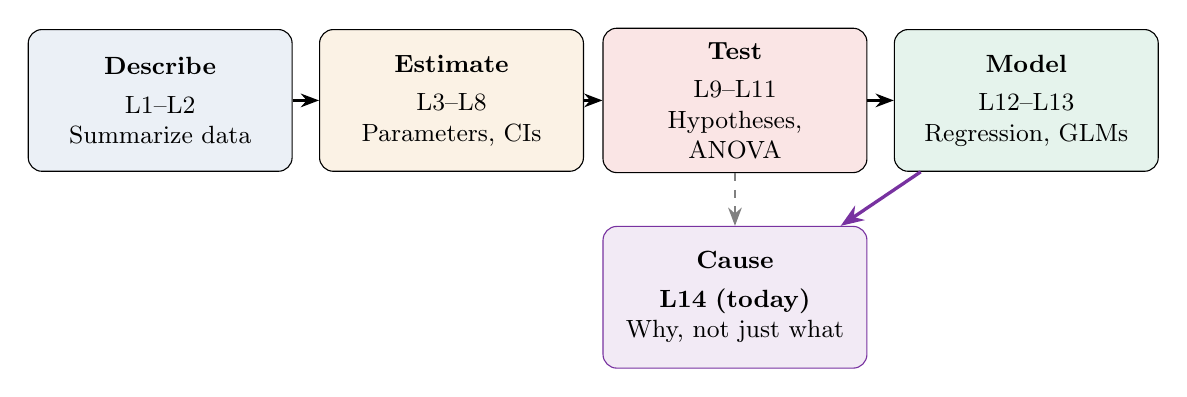
\begin{tikzpicture}[
  phase/.style={draw, rounded corners=5pt, text width=3cm, align=center, inner sep=5pt, font=\small, minimum height=1.8cm}
]
  \node[phase, fill=popblue!10] (desc) at (-5.5, 0) {
    \textbf{Describe}\\[3pt]
    L1--L2\\
    Summarize data
  };
  \node[phase, fill=orange1!10] (est) at (-1.8, 0) {
    \textbf{Estimate}\\[3pt]
    L3--L8\\
    Parameters, CIs
  };
  \node[phase, fill=sampred!10] (test) at (1.8, 0) {
    \textbf{Test}\\[3pt]
    L9--L11\\
    Hypotheses, ANOVA
  };
  \node[phase, fill=paramgreen!10] (model) at (5.5, 0) {
    \textbf{Model}\\[3pt]
    L12--L13\\
    Regression, GLMs
  };

  \draw[-{Stealth}, thick] (desc) -- (est);
  \draw[-{Stealth}, thick] (est) -- (test);
  \draw[-{Stealth}, thick] (test) -- (model);

  % Causal
  \node[draw=violet1, fill=violet1!10, rounded corners=5pt, text width=3cm, align=center, inner sep=5pt, font=\small, minimum height=1.8cm] (causal) at (1.8, -2.5) {
    \textbf{Cause}\\[3pt]
    \textbf{L14 (today)}\\
    Why, not just what
  };
  \draw[-{Stealth}, very thick, violet1] (model) -- (causal);
  \draw[-{Stealth}, thick, gray, dashed] (test) -- (causal);
\end{tikzpicture}
\end{center}
\end{frame}

% ============================================================
% PRACTICAL & HOMEWORK
% ============================================================
\begin{frame}
\frametitle{Practical Exercise}
\begin{center}
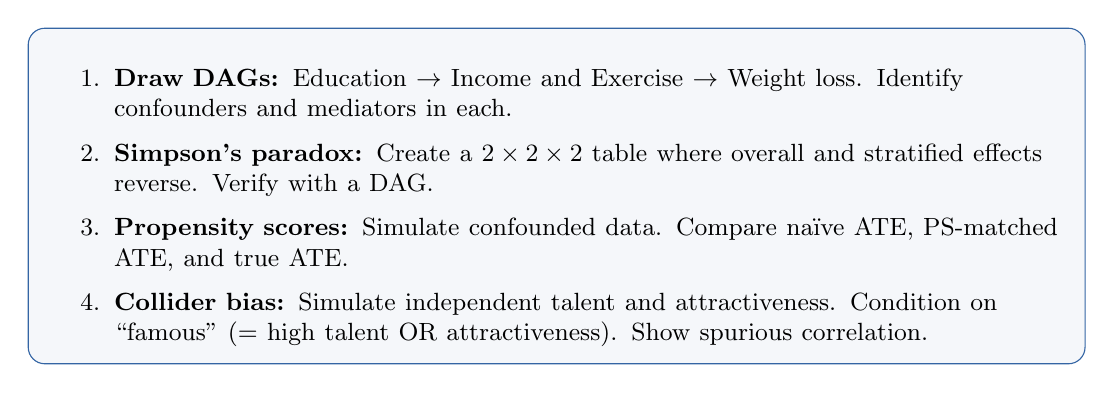
\begin{tikzpicture}
  \node[draw=popblue, fill=popblue!5, rounded corners=6pt, text width=13cm, align=left, inner sep=6pt] {
    \small
    \begin{enumerate}\setlength{\itemsep}{3pt}
      \item \textbf{Draw DAGs:} Education $\to$ Income and Exercise $\to$ Weight loss.
        Identify confounders and mediators in each.
      \item \textbf{Simpson's paradox:} Create a $2\times2\times2$ table where overall and stratified effects reverse. Verify with a DAG.
      \item \textbf{Propensity scores:} Simulate confounded data.
        Compare na\"ive ATE, PS-matched ATE, and true ATE.
      \item \textbf{Collider bias:} Simulate independent talent and attractiveness.
        Condition on ``famous'' ($=$ high talent OR attractiveness). Show spurious correlation.
    \end{enumerate}
  };
\end{tikzpicture}
\end{center}
\end{frame}

\begin{frame}
\frametitle{Homework}
\begin{enumerate}\setlength{\itemsep}{3pt}
  \item Surgery A has higher mortality than B in hospital data.
    (a) Draw a DAG with severity as confounder.
    (b) How would propensity scores estimate the causal effect?
    (c) What assumptions are needed?

  \item Users who see more ads buy more ($r = 0.4$, $p < 0.001$).
    (a) List three alternative explanations. (b) Draw DAGs for each.
    (c) Design an A/B test (from L11) to answer the causal question.

  \item Collider simulation: $X, Y \sim N(0,1)$ independent, $C = X + Y + \varepsilon$.
    (a) Compute $\text{cor}(X, Y)$. (b) Compute $\text{cor}(X, Y \mid C > 2)$. Explain.

  \item ``Distance to hospital'' as IV for ``receiving surgery.''
    Check each IV assumption. Which is hardest to defend?
\end{enumerate}
\end{frame}

\begin{frame}
\frametitle{Recommended Resources}

\begin{center}
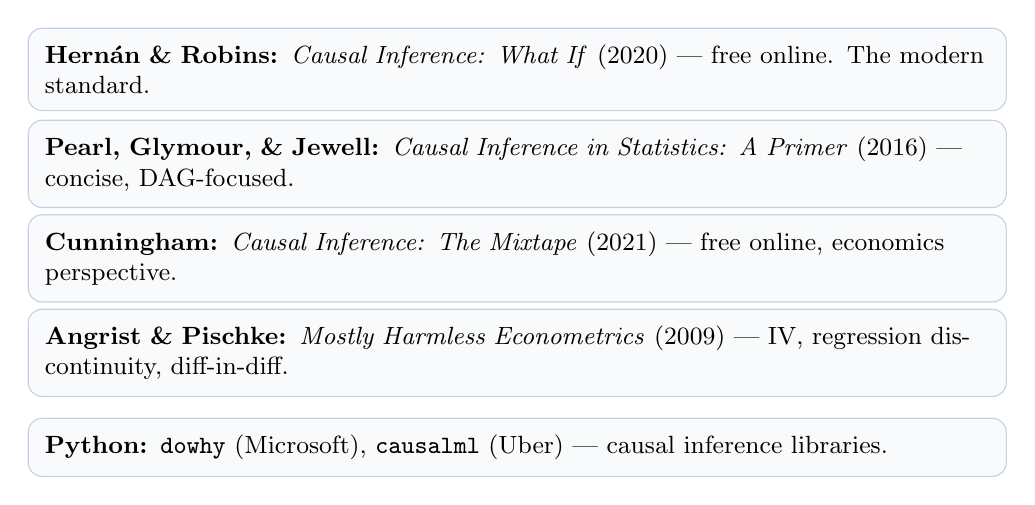
\begin{tikzpicture}[
  rbox/.style={draw=popblue!30, fill=popblue!3, rounded corners=5pt, text width=12cm, align=left, inner sep=6pt, font=\small}
]
  \node[rbox] at (0, 2.4) {
    \textbf{Hernán \& Robins:} \textit{Causal Inference: What If} (2020) --- free online. The modern standard.
  };
  \node[rbox] at (0, 1.2) {
    \textbf{Pearl, Glymour, \& Jewell:} \textit{Causal Inference in Statistics: A Primer} (2016) --- concise, DAG-focused.
  };
  \node[rbox] at (0, 0.0) {
    \textbf{Cunningham:} \textit{Causal Inference: The Mixtape} (2021) --- free online, economics perspective.
  };
  \node[rbox] at (0, -1.2) {
    \textbf{Angrist \& Pischke:} \textit{Mostly Harmless Econometrics} (2009) --- IV, regression discontinuity, diff-in-diff.
  };
  \node[rbox] at (0, -2.4) {
    \textbf{Python:} \texttt{dowhy} (Microsoft), \texttt{causalml} (Uber) --- causal inference libraries.
  };
\end{tikzpicture}
\end{center}
\end{frame}

% ============================================================
% CLOSING
% ============================================================
\begin{frame}
\begin{center}
  \vspace{2cm}
  {\Huge\bfseries\textcolor{popblue}{Questions?}}

  \vspace{1cm}
  {\large This concludes the Statistics lecture series.}

  \vspace{0.5cm}
  {\small L1--L14: From data description to causal inference.}
\end{center}
\end{frame}

\end{document}
